\documentclass[border=5pt]{standalone}
\usepackage[utf8]{inputenc}
\usepackage[T1]{fontenc}
\usepackage{tikz}
\usetikzlibrary{shapes.geometric,arrows.meta,positioning,calc}

\definecolor{eegcolor}{RGB}{66,133,244}
\definecolor{ragcolor}{RGB}{234,67,53}
\definecolor{fusioncolor}{RGB}{251,188,5}
\definecolor{llmcolor}{RGB}{52,168,83}

\begin{document}
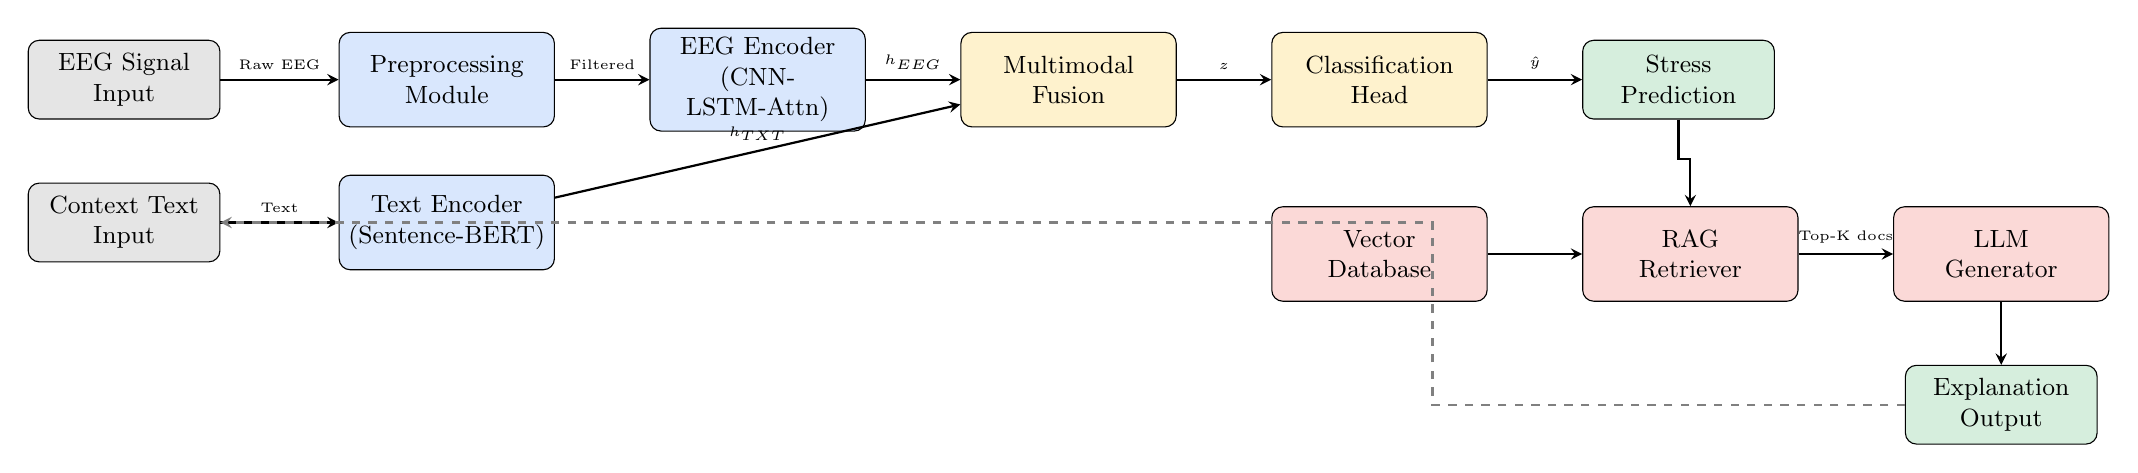
\begin{tikzpicture}[
    node distance=1.5cm,
    block/.style={rectangle, draw, fill=eegcolor!20, text width=2.5cm, text centered, rounded corners, minimum height=1.2cm, font=\small},
    inputblock/.style={rectangle, draw, fill=gray!20, text width=2.2cm, text centered, rounded corners, minimum height=1cm, font=\small},
    processblock/.style={rectangle, draw, fill=fusioncolor!20, text width=2.5cm, text centered, rounded corners, minimum height=1.2cm, font=\small},
    outputblock/.style={rectangle, draw, fill=llmcolor!20, text width=2.2cm, text centered, rounded corners, minimum height=1cm, font=\small},
    ragblock/.style={rectangle, draw, fill=ragcolor!20, text width=2.5cm, text centered, rounded corners, minimum height=1.2cm, font=\small},
    arrow/.style={->,>=stealth,thick},
    label/.style={font=\tiny, midway, above}
]

% Input Layer
\node[inputblock] (eeg_input) {EEG Signal\\Input};
\node[inputblock, below=0.8cm of eeg_input] (text_input) {Context Text\\Input};

% Processing Blocks
\node[block, right=1.5cm of eeg_input] (preprocess) {Preprocessing\\Module};
\node[block, right=1.2cm of preprocess] (encoder) {EEG Encoder\\(CNN-LSTM-Attn)};
\node[processblock, right=1.2cm of encoder] (fusion) {Multimodal\\Fusion};

% Text Encoder
\node[block, right=1.5cm of text_input] (text_enc) {Text Encoder\\(Sentence-BERT)};

% Classification
\node[processblock, right=1.2cm of fusion] (classifier) {Classification\\Head};
\node[outputblock, right=1.2cm of classifier] (output) {Stress\\Prediction};

% RAG Module
\node[ragblock, below=1cm of classifier] (vectordb) {Vector\\Database};
\node[ragblock, right=1.2cm of vectordb] (retriever) {RAG\\Retriever};
\node[ragblock, right=1.2cm of retriever] (llm) {LLM\\Generator};
\node[outputblock, below=0.8cm of llm] (explanation) {Explanation\\Output};

% Arrows with labels
\draw[arrow] (eeg_input) -- node[label] {Raw EEG} (preprocess);
\draw[arrow] (preprocess) -- node[label] {Filtered} (encoder);
\draw[arrow] (encoder) -- node[label] {$h_{EEG}$} (fusion);
\draw[arrow] (text_input) -- node[label] {Text} (text_enc);
\draw[arrow] (text_enc) -- node[label] {$h_{TXT}$} (fusion);
\draw[arrow] (fusion) -- node[label] {$z$} (classifier);
\draw[arrow] (classifier) -- node[label] {$\hat{y}$} (output);

% RAG Flow
\draw[arrow] (output.south) -- ++(0,-0.5) -| (retriever.north);
\draw[arrow] (vectordb) -- (retriever);
\draw[arrow] (retriever) -- node[label] {Top-K docs} (llm);
\draw[arrow] (llm) -- (explanation);

% Dashed feedback
\draw[arrow, dashed, gray] (explanation.west) -- ++(-6,0) |- (text_input.east);

\end{tikzpicture}
\end{document}
